\chapter{Theory}
\section{Higgs Phenomenology}

The Higgs sector of the Minimal Supersymmetric Standard Model (MSSM) consists of two SU (2) dou-
blets, H1 and H2 , whose relative contribution to electroweak symmetry breaking is determined by the
ratio of vacuum expectation values of their neutral components, tan β ≡ v2 /v1 . The spectrum of phys-
ical Higgs bosons is richer than in the SM, consisting of two neutral scalars h and H, one neutral pseu-
doscalar, A, and two charged scalars, H±. At the tree level, the mass matrix for the neutral scalars can be
expressed in terms of the parameters MZ , MA and tan β, and the mass of the lightest scalar h is bounded
from above by MZ . However, radiative corrections – especially those involving top and bottom quarks
and their supersymmetric partners, the stop and sbottom squarks – can significantly alter the tree-level
predictions for the Higgs-boson masses, and bring along a dependence on a large number of free pa-
rameters of the MSSM. While the CP symmetry is conserved at tree level in the MSSM Higgs sector,
radiative corrections can also introduce CP-violating phases, and induce mixing among all three neutral
states. In this report, however, we will focus on the CP-conserving case, by considering only real values
for the parameters in the soft SUSY-breaking Lagrangian and for the Higgs mass μ in the superpotential.
In general, the couplings of the MSSM Higgs bosons to gauge bosons and matter fermions dif-
fer from those of the SM Higgs. However, in large regions of the MSSM parameter space one of the
scalars has SM-like couplings, while the other Higgs bosons are decoupled from the gauge bosons, and
their couplings to down-type (up-type) fermions are enhanced (suppressed) by tan β. As in the SM,
gluon fusion is one of the most important production mechanisms for the neutral Higgs bosons, whose
couplings to the gluons are mediated by the top and bottom quarks and their superpartners. However,
for intermediate to large values of tan β the associated production with bottom quarks can become the
dominant production mechanism for the neutral Higgs bosons that have enhanced couplings to down-
type fermions. The production of the charged Higgs H±, on the other hand, proceeds mainly through
its coupling to a top-bottom pair. A sufficiently light H± is produced in the decay of a top quark, and it
decays dominantly in a tau-neutrino pair. A heavy H± is produced in association with a top quark and it
decays dominantly in a top-bottom pair.
The discovery by ATLAS and CMS of what appears to be a neutral scalar with mass around
125.5 GeV [1, 2] puts the studies of the Higgs sector of the MSSM in an entirely new perspective. In
order to remain viable, a point in the MSSM parameter space must now not only pass all the (ever
stricter) experimental bounds on superparticle masses, but also lead to the prediction of a scalar with
mass, production cross section and decay rates compatible with those measured at the LHC. In particular,
the relatively large mass of the roughly-SM-like scalar discovered at the LHC implies either very heavy
stops, of the order of 3 TeV, or a large value of the left-right stop mixing term (see, e.g., Refs. [648,649]).
The “benchmark scenarios” routinely considered in MSSM studies had been devised when the Higgs
sector was constrained only by the LEP searches, and many of them, such as the so-called “no-mixing”
scenario, are now ruled out because they predict a too-light SM-like scalar. Others, such as the so-called
mmax scenario, are constrained for the opposite reason, i.e. they can predict a too-heavy SM-like scalar.
h
To address the need for new benchmark scenarios to be used in future studies of the MSSM Higgs sector,
in Section 14.2 we will define scenarios that are compatible both with the properties of the Higgs boson
discovered at the LHC and with the current bounds on superparticle masses.
The fact that information on the Higgs boson mass, production and decays has now become avail-
able also puts new emphasis on the need for accurate theoretical predictions of those quantities. In the
studies presented in this report, the masses and mixing of the MSSM Higgs bosons are computed with
the public code F EYN H IGGS [24–27], which implements the full one-loop radiative corrections together
with the dominant two-loop effects. The theoretical accuracy of the prediction of F EYN H IGGS for the

lightest-scalar mass was estimated to be of the order of 3 GeV [26, 650, 651], i.e., already comparable
to the accuracy of the mass measurement at the LHC. Improving the accuracy of the theoretical predic-
tion for the MSSM Higgs masses will require the inclusion in public computer codes of the remaining
two-loop effects [652–654] and at least the dominant three-loop effects [655–657].
The production and decay rates of a SM-like Higgs boson in the MSSM are sensitive to contri-
butions from virtual SUSY particles, and their measurement at the LHC – combined with the searches
for additional Higgs bosons – can be used to constrain the MSSM parameter space. To this effect, the
theoretical predictions for cross section and decays must include precise computations of the SUSY con-
tributions. In Section 14.3 we use the public code S US H I [641] and the POWHEG implementation of
Ref. [77] to compute the total and differential cross sections for neutral Higgs-boson production in gluon
fusion, including a NLO-QCD calculation of quark and squark contributions plus higher-order quark
contributions adapted from the SM calculation. We show that the SUSY contributions can be sizeable in
regions of the MSSM parameter space where the third-generation squarks are relatively light, and discuss
the theoretical uncertainty of the predictions for the cross sections.
Finally, we study and update the exclusion limits on light charged MSSM Higgs bosons in the
(MH± , tan β)-plane in various benchmark scenarios in Section 14.4. Particular emphasis is placed on
the dependence of the limits on the variation of SUSY parameters. We also provide improved NLO-
QCD cross section predictions for heavy charged Higgs production in the so-called four and five-flavor
schemes in Section 14.5. The five-flavor scheme cross section is calculated with a new scheme for setting
the factorization scale and takes into account the theoretical uncertainty from scale variation and the PDF,
αs and bottom-mass error. We observe good agreement between the 4FS and 5FS NLO-calculations and
provide a combined prediction following the Santander matching.
14.2
New MSSM benchmark scenarios
Within the MSSM an obvious possibility is to interpret the new state at about 125.5 GeV as the light
CP-even Higgs boson [334, 338, 648, 649, 658–662]. At the same time, the search for the other Higgs
bosons has continued. The non-observation of any additional state in the other Higgs search channels
puts by now stringent constraints on the MSSM parameter space, in particular on the values of the tree-
level parameters MA (or MH± ) and tan β. Similarly, the non-observation of supersymmetric (SUSY)
particles puts relevant constraints on the masses of the first and second generation scalar quarks and the
gluino, and to lesser degree on the stop and sbottom masses (see Refs. [663, 664] for a recent summary).
Due to the large number of free parameters, a complete scan of the MSSM parameter space is
impractical in experimental analyses and phenomenological studies. Therefore, the Higgs search results
at LEP were interpreted [458] in several benchmark scenarios [16, 665]. In these scenarios only the two
parameters that enter the Higgs sector tree-level predictions, MA and tan β, are varied (and the results are
usually displayed in the MA − tan β plane), whereas the other SUSY parameters, entering via radiative
corrections, are fixed to particular benchmark values which are chosen to exhibit certain features of the
MSSM Higgs phenomenology. These scenarios were also employed for the MSSM Higgs searches at
the Tevatron and at the LHC.
By now, most of the parameter space of the original benchmark scenarios [16, 665] has been
ruled out by the requirement that one of the CP-even Higgs boson masses should be around 125.5 GeV.
Consequently, new scenarios have been proposed [31], which are defined such that over large parts of
their available parameter space the observed signal at about 125.5 GeV can be interpreted in terms of
one of the (neutral) Higgs bosons, while the scenarios exhibit interesting phenomenology for the MSSM
Higgs sector. The benchmark scenarios are all specified using low-energy MSSM parameters, i.e. no
particular soft SUSY-breaking scenario was assumed. Constraints from direct searches for Higgs bosons
are taken into account, whereas indirect constraints from requiring the correct cold dark matter density,
BR(b → sγ), BR(Bs → μ+ μ− ) or (g−2)μ are neglected. However interesting, those constraints de

\begin{figure}[tp]
     \begin{center}

            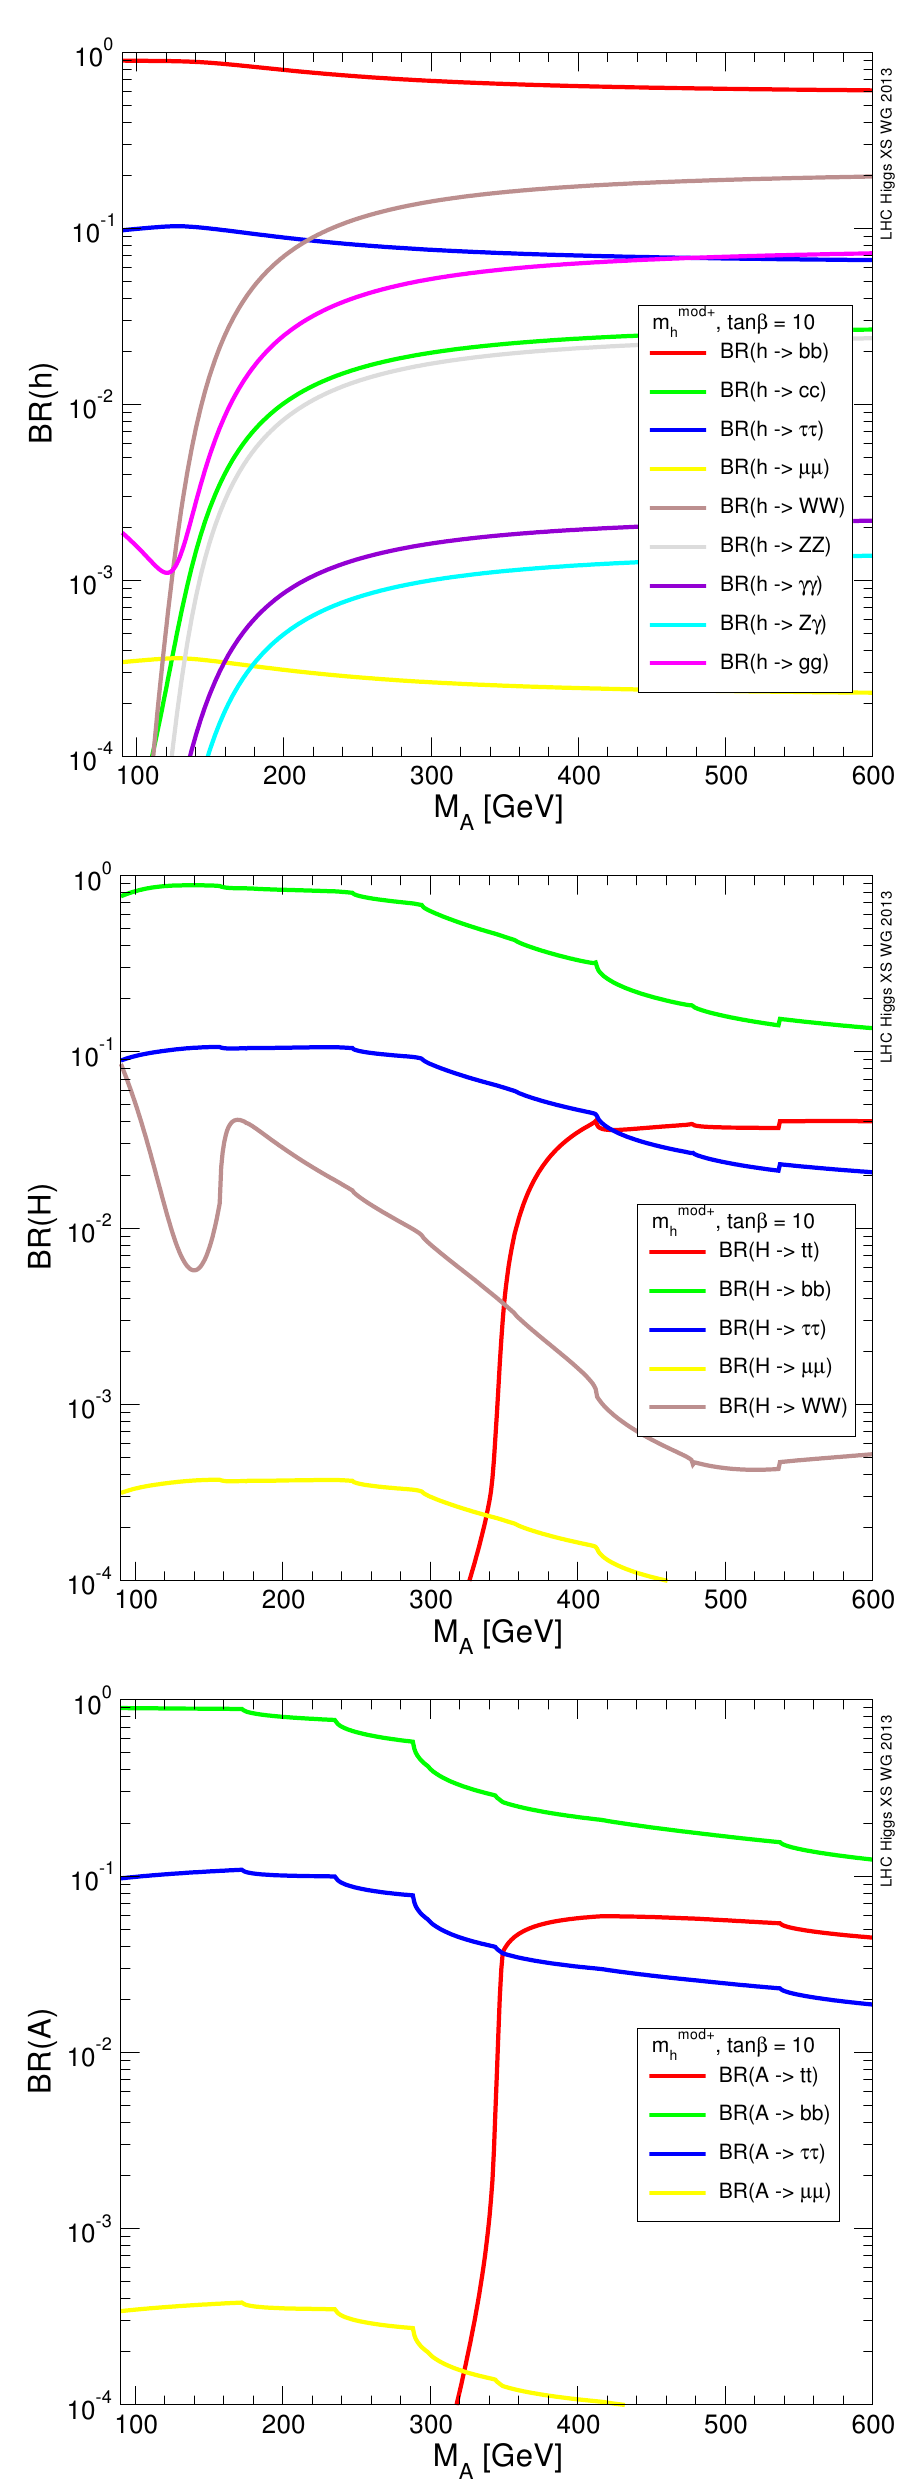
\includegraphics[width=0.5\textwidth]{figure/br.png}

    \end{center}
    \caption{Branching fraction for the MSSM neutral higgses $h/H/A$ in the $m_h^{mod+}$ scenario.}
   \label{fig:br}

\end{figure}

In the MSSM for large region of parameter space one found that one of the 
$CP$-even neutral Higgses  has properties that resemble the one of the SM Higgs,
this is usually the case for the lightest Higgs, \emph{h}, the other two, $H$ and $A$, 
tend to be degenerate in mass and decouple from gauge bosons.
An interesting fenomenological consequence is that the coupling of the latter
two Higgses with down (up) type fermions are enhanced
(suppressed) by $\tan\beta$, meaning that for large $\tan\beta$
bottom-quark and $\tau$ lepton will play a more important role than in
the SM case either for production and decay.

The production of the neutral $CP$-even MSSM Higgs bosons at hadron
colliders proceeds via the same processes as for the SM Higgs
production. However, the pseudoscalar $A$ instead cannot be produced
in association with gauge bosons or in vector boson fusion (VBF) at
tree-level, as this coupling is forbidden due to $CP$-invariance.  At
the LHC one of the most relevant production mechanisms for the MSSM
Higgs bosons is gluon-gluon fusion, $gg\rightarrow A/H/h$. In
addition, the production in association with $b$-quarks becomes
important for large value of $\tan\beta$. Those are the two production mechanism
that are considered in this analysis, Figure~\ref{fig:prod} shows the Feynman-diagram
for those processes, while Figure~\ref{fig:xsec} shows the production cross section of the neutral 
MSSM Higgses via these two processes. The search is divided in two category which are optimized
for the two different production mode considered, in the gluon-fusion category
is requred a b-jet veto (for definition of b-tagging algorithm see chapter~\ref{chap:detector}), in fact no b-jet in the final state are present for this
production mode. In contrast a a b-jet tag is required for b-associated production,
this category is expected to be very sensitive to $\tan\beta$. The two category are
ortogonal and present different backgrounds contributions, which can be
optimized separately. 


The decays of the neutral
MSSM Higgs bosons (in the assumption that all supersymmetric particle
are heavy enough) are the same as for the SM one with the already
cited exception of $A$. Figure~\ref{fig:xsec} shows the decay branching fractions
for $H$ and $A$ as a function of the mass, 
the decay into tau pair is the most important after $b\bar{b}$ and the one used in this analysis. The 
decay channel in $b\bar{b}$ is in fact very challenging due to the huge background from
QCD multi-jet.
In this thesis only cases in which the taus decay one in $e + 2\nu$ and
the other in $\mu + 2\nu$ are considered, This final state corresponds to a total
$\tau^+\tau^-$ branching ratio of approximately 6\%.

\begin{figure}[tp]
     \begin{center}

            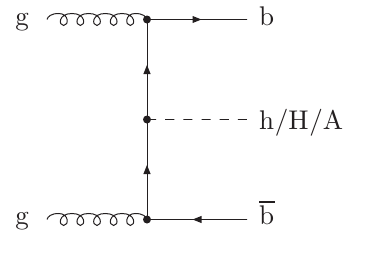
\includegraphics[height=3cm]{figure/bba.png}
            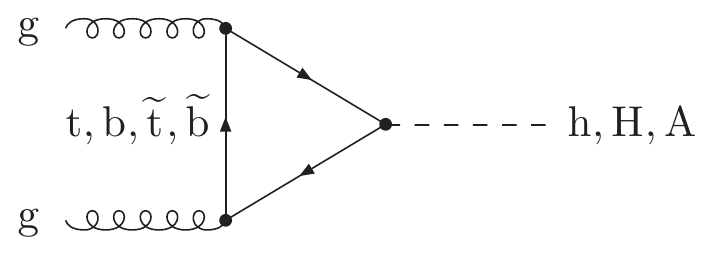
\includegraphics[height=3cm]{figure/ggf.png}

    \end{center}
    \caption{Feynman diagram for b-associated production and gluon-gluon fusion for MSSM neutral Higgs.}
   \label{fig:prod}
\end{figure}

\begin{figure}[tp]
     \begin{center}

            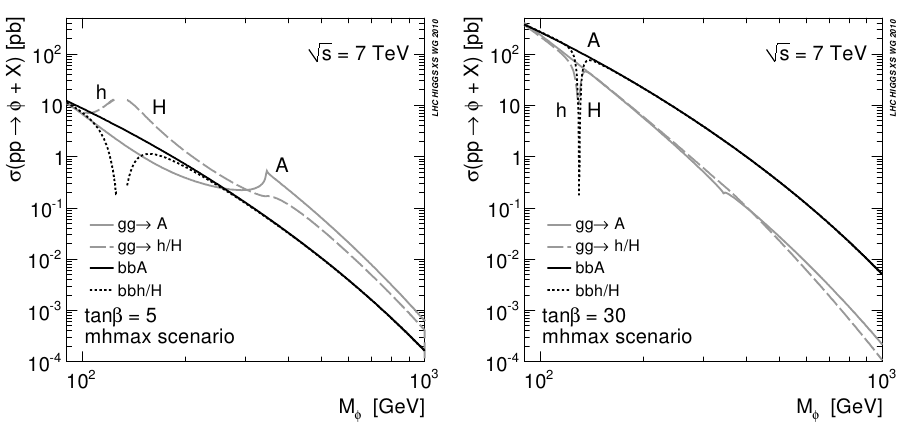
\includegraphics[width=\textwidth]{figure/xsec.png}

    \end{center}
    \caption{Production cross section for the \emph{h/H/A} MSSM neutral Higgs bosons via b-associated production and
	gluon-gluon fusion production mode. The calculation are for the $m_h^{max}$ scenario and for $\tan \beta=5$ (left) and $\tan \beta=30$ (right).}
   \label{fig:xsec}
\end{figure}
